% ----------------------------------------------------------------------
% Authors:     Tomas Fryza, Wykys
%              Dept. of Radio Electronics, Brno Univ. of Technology
% Created:     2018-05-22
% Last update: 2019-07-24
% Description: Template using official colors of Brno University of 
% Technology defined by graphical manual in 2015.
% ----------------------------------------------------------------------
% License:     CC BY-NC-SA 4.0
% Keep the name of the authors. You may not use the template for 
% commercial purposes. Share and modify as you like under the same 
% license as the original. 
%
% https://creativecommons.org/licenses/by-nc-sa/4.0/
% ----------------------------------------------------------------------

% ----------------------------------------------------------------------
% PACKAGES
% ----------------------------------------------------------------------

%% Sets aspect ratio to 16:10, and frame size to 160mm by 100mm
% Please, do not use old-school 4:3 ratio anymore:)
\documentclass[aspectratio=1610]{beamer}

%% Select your favorite language
\usepackage[francais]{babel} % Multilingual support for LaTeX
% \usepackage[czech]{babel}

\usepackage[utf8]{inputenc} % Accept different input encodings
\usepackage{ucs} % Extended UTF-8 input encoding support for LaTeX
\usepackage{graphicx} % Enhanced support for graphics
\usepackage{listings} % Typeset source code listings using LaTeX
\usepackage{color} % Colour control for LaTeX documents
\usepackage{subcaption}
%% Copy your favorite logo from "vut_logo_archive/" to root folder 
% and rename file to "logo.png"
\usepackage{listings}

%% Select color theme
\usepackage{themevut} % All in red:)
% \usepackage[FA]{themevut}
% \usepackage[FAST]{themevut}
% \usepackage[FaVU]{themevut}
% \usepackage[FCH]{themevut}
% \usepackage[FEKT]{themevut}
% \usepackage[FIT]{themevut}
% \usepackage[FP]{themevut}
% \usepackage[FSI]{themevut}
% \usepackage[CESA]{themevut}
% \usepackage[USI]{themevut}

% ----------------------------------------------------------------------
% TITLE PAGE
% ----------------------------------------------------------------------

% The short title appears at the bottom of every slide, the full title
% is only on the title page.
\title[HMMA307]
{Modèles linéaires généralisés sur données de comptages}

% Type of project, i.e. Bachelor, Master, PhD, etc.
\subtitle
{Master 2 MIND}

% Your name
\author[]
{Ryma Lakehal}

% Your institution
\institute
{Faculté des sciences \\
Université de Montpellier
}

% Date, can be changed to a custom date
\date{\today}

% Logo on title page
\titlegraphic{
\includegraphics[height=1.5cm]{UM_Logo}
\includegraphics[height=1.5cm]{fds}}

\begin{document}

% ----------------------------------------------------------------------
% PRESENTATION SLIDES
% ----------------------------------------------------------------------

\begin{frame}
    % Print the title page as the first slide
    \titlepage
\end{frame}

\section*{Contents}

\begin{frame}
\frametitle{Plan}
  \tableofcontents
\end{frame}




\section[Intro]{Introduction}
\begin{frame}{Introduction}
\begin{itemize}
    \item Régression de Poisson
    \item Régression binomiale négative
\end{itemize}

\begin{block}{}
Pourquoi ces modèles ?
\end{block}

\begin{itemize}
    \item Les modèles linéaires classiques ne sont pas adaptés pour analyser des variables à expliquer (ou réponses) de type “comptage”.
    \begin{align*}
y_i &= \beta_0 + \beta_1 x_i + \varepsilon_i \\
\varepsilon &\sim N(0, \sigma)
\end{align*}
    \item Les données de type comptage ne sont pas distribuées selon une loi Normale.
    \item La variance des résidus n’est pas constante mais proportionnelle aux comptages moyens prédits par le modèle.
\end{itemize}

\end{frame}

%	\begin{frame}[plain]
%		\maketitle
%	\end{frame}
\section{Le modèle linéaire généralisé}

\begin{frame}{Le modèle linéaire généralisé} 
\begin{align*}
y_i &\sim N(\mu_i, \sigma)\\
\mathrm{E}(Y|X) &= \mu\\
\mu_i &= \beta_0 + \beta_1 x_i
\end{align*}

Ces modèles sont constitués de trois éléments :
	
\begin{itemize}
	    \item un prédicteur linéaire,
	    $\eta=\mathbf{X}\boldsymbol{\beta}$
        \item  une distribution de probabilité de la famille exponentielle $y_i \sim \mathrm{Prob}(\mu_i)$
        \item une fonction de lien \eta_i = g(\mu_i)$
\end{itemize}
\end{frame}





%\subsection{Validité d'un modèle linéaire généralisé}
%\begin{frame}{Validité d'un modèle linéaire généralisé} 

	
%\end{frame}


\section{Données \texttt{Parastism}}
\subsection{Présentation des données \texttt{Parastism}}
\begin{frame}{Présentation des données \texttt{Parastism}}
\begin{itemize}
    \item 196 fruits contient au moins un parasitoïde vivant ou éradiqué
    \item 63 fruits non infectés "contrôlés"
    \item 67 fruits avec le parasite \textit{A. melinus} sans sucre
    \item 66 fruits infectés du même parasite plus le sucre
    \item au total : 949 parasitoïdesvivants et 365 parasites éliminés contenant un œuf ou larves d’Aphytis.
    
\end{itemize}

\begin{figure}[!h]
    \centering
    \begin{subfigure}[b]{0.5\textwidth}
        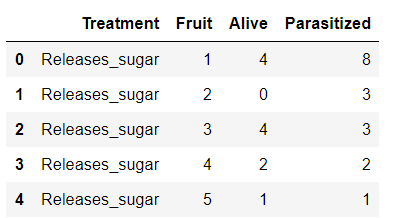
\includegraphics[width=\textwidth]{datahead.png}
    \end{subfigure}
    \begin{subfigure}[b]{0.4\textwidth}
        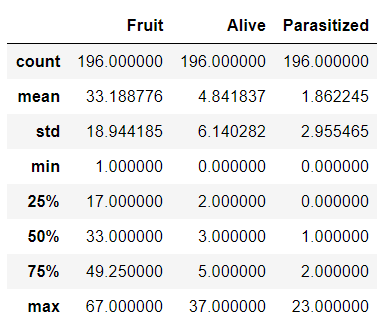
\includegraphics[width=\textwidth]{datadescribe.png}
    \end{subfigure}
    
\end{figure}	

\end{frame}

\subsection{Visualisation des \texttt{Parastism}}
\begin{frame}{Visualisation des données \texttt{Parastism}}
 \begin{figure}[h]
\centering
 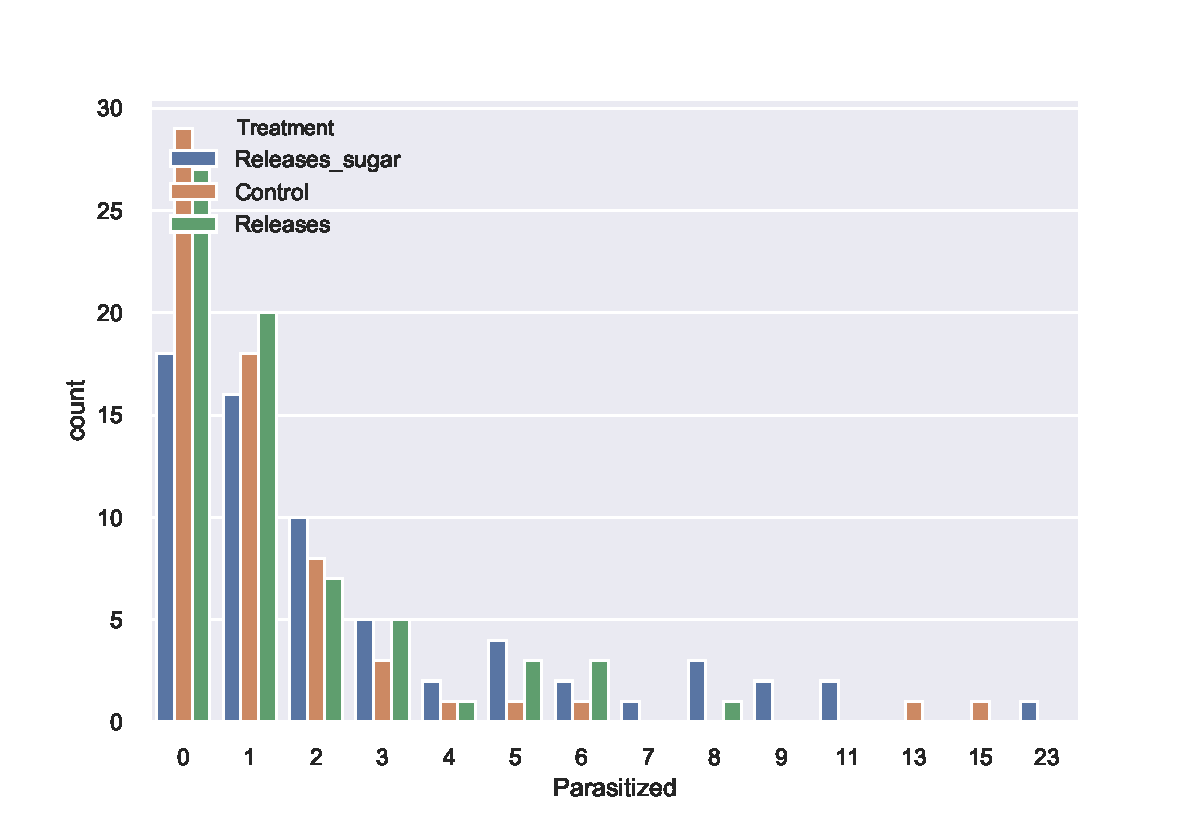
\includegraphics[width=.7\textwidth]{Histogram of the count.pdf}
 \caption{Histogramme des traitements en fonction de la variable \texttt{Parasitized} } 
 \label{hist_para}
 \end{figure}

\end{frame}




\section{Modèle linéaire classique}
\subsection{Normalité des résidus}
\begin{frame}{Modèlisation linéaire}

Le modèle :
\begin{align*}
Parasitized_i &= \beta_0 + \beta_1 Control_i + \beta_2 Realises_i + \beta_3 Realises\_sugar_i + \varepsilon_i \\
\varepsilon &\sim N(0, \sigma)
\tag{3}
\end{align*}

\begin{figure}[h]
\centering
 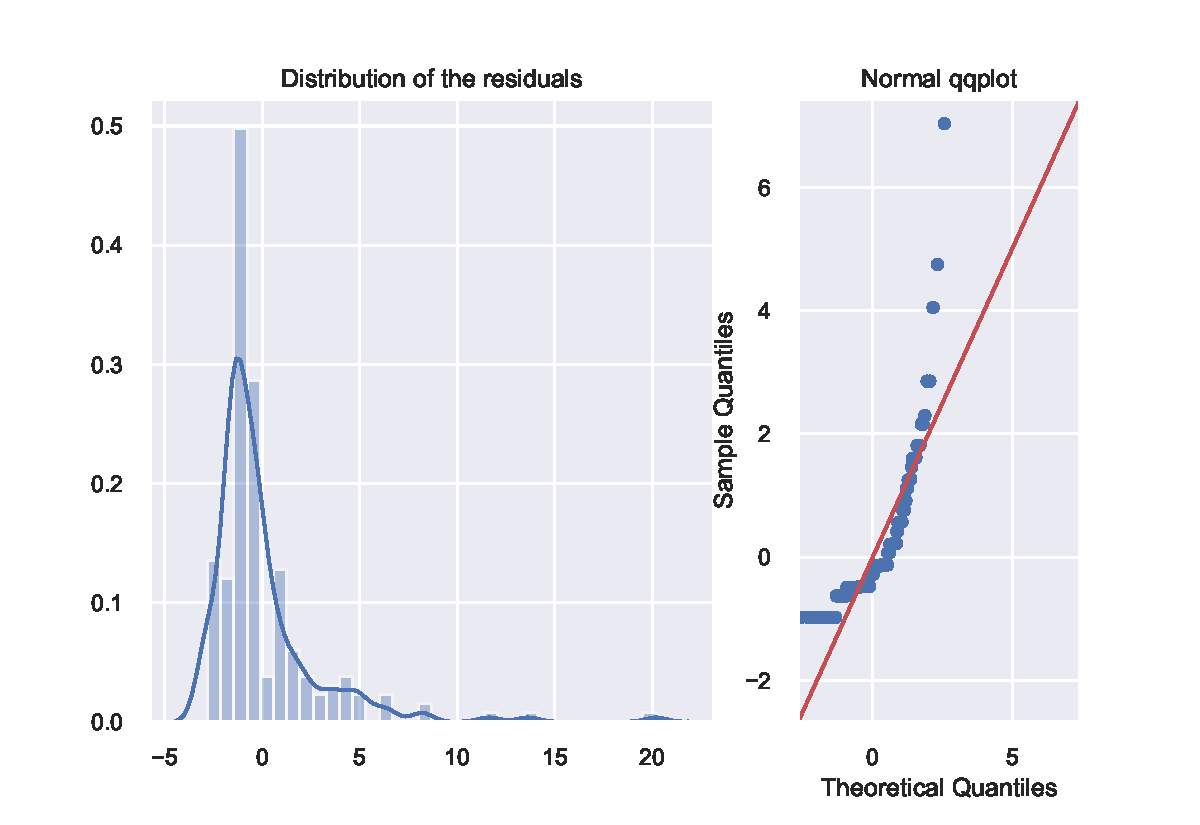
\includegraphics[width=.5\textwidth]{Distribution and normal QQ plot residuals .pdf}
 \caption{Distribution et normal Q-Q plot des résidus du modèle linéaire ajusté} 
 \label{norm_qq}
 \end{figure}

\end{frame}


\subsection{Homoscédasticité}
\begin{frame}{Homoscédasticité - scale-location plot}

\begin{figure}[h]
\centering
 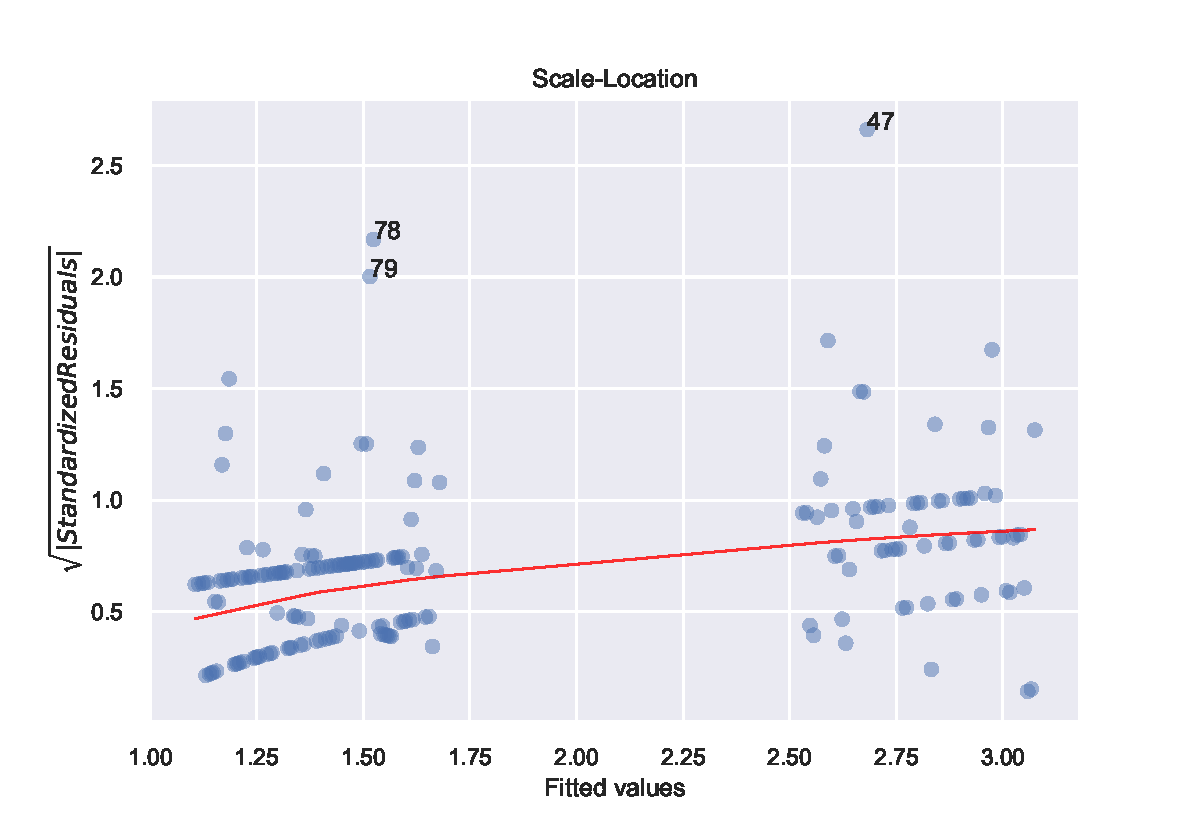
\includegraphics[width=.7\textwidth]{scale-location plot.pdf}
 \caption{scale-location plot pour vérifier l'homoscédasticité} 
 \label{homosc}
 \end{figure}
\end{frame}

\section{Régression de Poisson}
\subsection{Ajustement du modèle de régression linéaire de Poisson aux donnéesParastism}
\begin{frame}{Régression de Poisson}
Le modèle est : 

\begin{align*}
Parasitized_i &\sim Poisson(\mu_i)\\
\mathrm{E}({Parasitized|Treatment}) &= \mu\\
\mu_i &= \mathrm{exp}(\eta_i)\\
\eta_i &= \beta_0 + \beta_1 Control_i + \beta_2 Realises_i + \beta_3 Realises\_sugar_i
\end{align*}



L’ajustement est réalisé à l’aide de la fonction \textbf{Poisson.fit} du module \textbf{statsmodels} 
\end{frame}


\begin{frame}{Régression de Poisson}
\begin{figure}[h]
\centering
 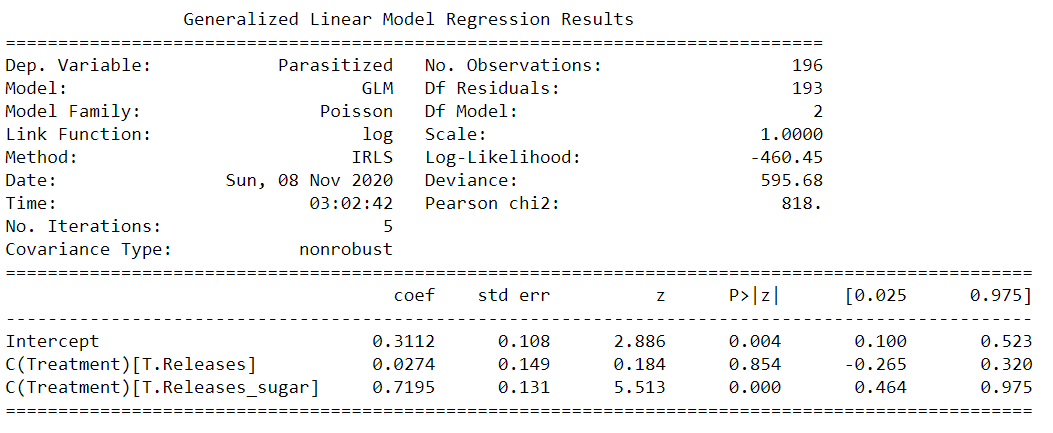
\includegraphics[width=.8\textwidth]{poisson.fit.png}

 \end{figure}
Le ratio residual deviance/ddl est égal à 5304.4/193, soit 27,48. Ce ratio est très largement supérieur à 1 et ce qui permet de mettre en évidence la présence d’une surdispersion
\end{frame}



\section{Régression binomiale négative}
\subsection{Ajustement du modèle de régression binomiale négative aux donnéesParastism}
\begin{frame}{Ajustement du modèle de régression binomiale négative aux donnéesParastism}

\begin{align*}
Parasitized_i &\sim NB(\mu, k)\\
\mathrm{E}({Parasitized|Treatment}) &= \mu\\
\mu_i &= \mathrm{exp}(\eta_i)\\
\eta_i &= \beta_0 + \beta_1 Control_i + \beta_2 Realises_i + \beta_3 Realises\_sugar_i
\end{align*}

\begin{figure}[h]
\centering
 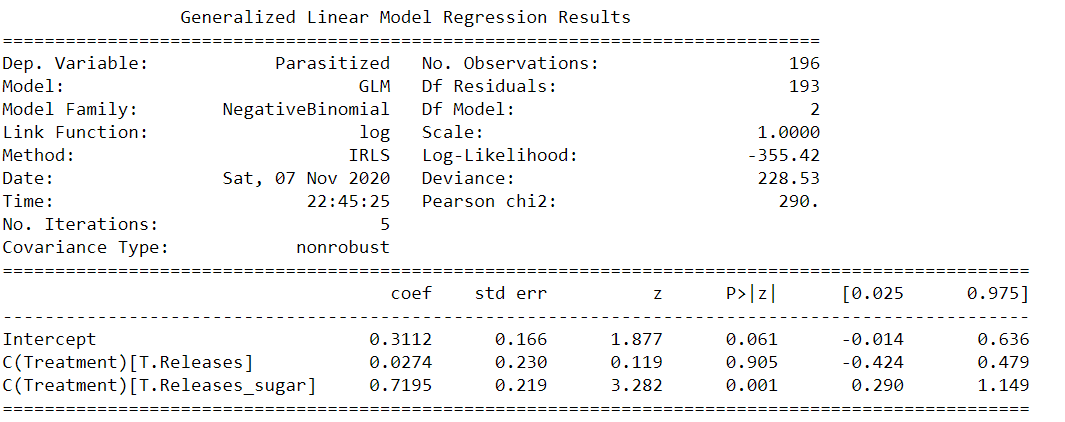
\includegraphics[width=.7\textwidth]{NB.fit.png}

 \end{figure}
Le ratio residual deviance/ddl est égal à 1.18

\end{frame}

\subsection{Calculs des effets marginaux}
\begin{frame}{Calculs des effets marginaux}
Les effets marginaux sont utilisées pour décrire l’impact d’un prédicteur sur la variable à expliquer. 

On s'intéresse aux effects marginaux moyen, pour ce faire, on a la fonction \textbf{.get\_margeff()} de la bibliothèque \textbf{Statsmodels}.

 \begin{figure}[h]
\centering
 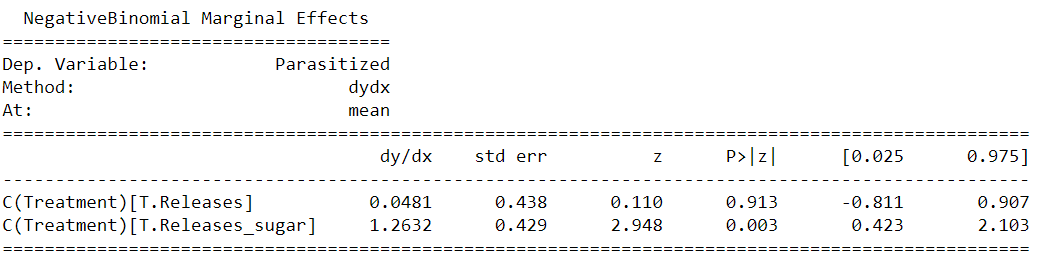
\includegraphics[width=1\textwidth]{marginal effects.png}

 \end{figure}  
 
 La valeur de \textbf{Releases\_sugar} est 1.26 ce qui peut être interprété que quand la valeur de \textbf{Releases\_sugar} augmente d'une unité, la probabilité des parasitoïdes éliminé ou le taux de parasitism augmente de 126\%.
\end{frame}

\section{conclusion}
\begin{frame}{Conclusion}
En appliquant les différents modèles de modélisation, nous avons constaté que le modèle linéaire généralisé de distribution binomiale négative est celui qui s'adapte le mieux à notre jeu de données \textbf{Parastism}.
Et de ce dernier modèle, on conclut que les provisions de sucre aident les parasitoïdes à maintenir leurs réserves de sucre ce qui fera augmenter leurs fécondités et ainsi le taux de parasitisme (\texttt{Parasitism})

\end{frame}



\end{document}
